
%%%%%%%%%%%%%%%%%%%%%%%%%%%%%%%%%%%%%
% [x] Removed we
% [x] Tidied up language



\paragraph{Reductions}
The current reduction is not the most optimal choice. Rather than a single work-item summing up all the values, this could be done by multiple work-items. Using a binary sum allows us to do this. An example of this can be seen in Figure~\ref{fig:binary-reduction}

\begin{figure}[ht]
\centering
% This file was created by tikzplotlib v0.8.7.
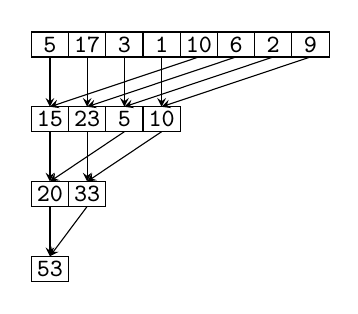
\begin{tikzpicture}

\definecolor{color0}{rgb}{1,0.498039215686275,0.0549019607843137}
\definecolor{color1}{rgb}{0.172549019607843,0.627450980392157,0.172549019607843}

\begin{axis}[
legend cell align={left},
legend style={fill opacity=0.8, draw opacity=1, text opacity=1, draw=white!80.0!black},
tick align=outside,
tick pos=left,
x grid style={white!69.01960784313725!black},
xlabel={Runtime (s)},
xmin=-9.5, xmax=19.5,
xtick style={color=black},
ymin=-3, ymax=15,
hide axis
]

% Array of 8
% \draw (1,10) rectangle (17,11);
\draw (1,10) rectangle (3,11);
\node[] at (axis cs: 2,10.5) {\small\texttt{5}};
\draw[->,>=stealth] (2,10) to (2, 8);
\draw (3,10) rectangle (5,11);
\node[] at (axis cs: 4,10.5) {\small\texttt{17}};
\draw[->,>=stealth] (4,10) to (4, 8);
\draw (5,10) rectangle (7,11);
\node[] at (axis cs: 6,10.5) {\small\texttt{3}};
\draw[->,>=stealth] (6,10) to (6, 8);
\draw (7,10) rectangle (9,11);
\node[] at (axis cs: 8,10.5) {\small\texttt{1}};
\draw[->,>=stealth] (8,10) to (8, 8);

\draw (9,10) rectangle (11,11);
\node[] at (axis cs: 10,10.5) {\small\texttt{10}};
\draw[->,>=stealth] (10,10) to (2,8);
% \draw[->,>=stealth] plot [smooth,tension=1] coordinates {(10,10) (8.333,9.333) (4.333,8.666) (2,8)};
\draw (11,10) rectangle (13,11);
\node[] at (axis cs: 12,10.5) {\small\texttt{6}};
\draw[->,>=stealth] (12,10) to (4,8);
% \draw[->,>=stealth] plot [smooth,tension=1] coordinates {(12,10) (10.333,9.333) (6.333,8.666) (4,8)};
\draw (13,10) rectangle (15,11);
\node[] at (axis cs: 14,10.5) {\small\texttt{2}};
\draw[->,>=stealth] (14,10) to (6,8);
% \draw[->,>=stealth] plot [smooth,tension=1] coordinates {(14,10) (12.333,9.333) (8.333,8.666) (6,8)};
\draw (15,10) rectangle (17,11);
\node[] at (axis cs: 16,10.5) {\small\texttt{9}};
\draw[->,>=stealth] (16,10) to (8,8);
% \draw[->,>=stealth] plot [smooth,tension=1] coordinates {(16,10) (14.333,9.333) (10.333,8.666) (8,8)};


% Array of 4
\draw (1,7) rectangle (3,8);
\node[] at (axis cs: 2,7.5) {\small\texttt{15}};
\draw[->,>=stealth] (2,7) to (2, 5);
\draw (3,7) rectangle (5,8);
\node[] at (axis cs: 4,7.5) {\small\texttt{23}};
\draw[->,>=stealth] (4,7) to (4, 5);
\draw (5,7) rectangle (7,8);
\node[] at (axis cs: 6,7.5) {\small\texttt{5}};
\draw[->,>=stealth] (6,7) to (2,5);
% \draw[->,>=stealth] plot [smooth,tension=1] coordinates {(6,7) (5.333,6.333) (3.333,5.666) (2,5)};
\draw (7,7) rectangle (9,8);
\node[] at (axis cs: 8,7.5) {\small\texttt{10}};
\draw[->,>=stealth] (8,7) to (4,5);
% \draw[->,>=stealth] plot [smooth,tension=1] coordinates {(8,7) (7.333,6.333) (5.333,5.666) (4,5)};


% Array of 2
\draw (1,4) rectangle (3,5);
\node[] at (axis cs: 2,4.5) {\small\texttt{20}};
\draw[->,>=stealth] (2,4) to (2, 2);
\draw (3,4) rectangle (5,5);
\node[] at (axis cs: 4,4.5) {\small\texttt{33}};
\draw[->,>=stealth] (4,4) to (2, 2);
% \draw[->,>=stealth] plot [smooth,tension=1] coordinates {(4,4) (3.666,3.333) (2.666,2.666) (2,2)};

% Array of 1
\draw (1,1) rectangle (3,2);
\node[] at (axis cs: 2,1.5) {\small\texttt{53}};


% \draw[->,>=stealth] (-1.5,7) to[bend right=-60] (2.5, 7);
% \draw[->,>=stealth] (8.5,7) to[bend right=-60] (12.5, 7);

% \draw[->,>=stealth] (1.5,1) to[bend right=-60] (-2.5, 1);
% \draw[->,>=stealth] (11.5,1) to[bend right=-60] (7.5, 1);

% \addplot [color0, forget plot]
% table {%
% 0.009462 0.925
% 0.009462 1.075
% };
\end{axis}

\end{tikzpicture}

\vspace{-3mm}
\caption{Binary Reduction.}
\label{fig:binary-reduction}
\vspace{-2mm}
\end{figure}


Additionally, every iteration \texttt{tot\_cells} is reduced. However this is constant throughout all iterations. Therefore this only needs to reduced this once.  The speeds achieved for each type of reduction, with only \texttt{tot\_u} reduced can be seen in Table~\ref{table:reductions}.


\begin{table}[ht]
\vspace{-5mm}
\centering
\caption{Runtimes of both types of kernels, without the \texttt{tot\_cells} reduction.}
\vspace{1mm}
\begin{tabular}{|c||p{4.8em}|p{5em}|}
    \hline
    & \multicolumn{2}{|c|}{Runtime (s)}\\
    \hline
    Size & Local Memory & Binary Reduction \\
    \hline
    128x128 & 0.990 & 0.958 \\
    \hline
    256x256 & 2.664 & 2.529 \\
    \hline
    1024x1024 & 3.696 & 3.655 \\
    \hline
\end{tabular}
\label{table:reductions}
\vspace{-1mm}
\end{table}

There is a further optimisation that can be made. The reduction values are only required at the end of the simulation. The work-group sums can be stored for all iterations. These can all be summed up on the device after all iterations have completed, then copied back to the host as an array of \texttt{av\_vels}. This helps since partial sums no longer need to be copied back from the device every iteration. The \texttt{clEnqueueReadBuffer} command is a blocking command. This produces a problem that is similar to the issue with \texttt{clFinish} previously identified. This stops the next kernel from being queued until the memory has been copied from the device. The speedup gained from this can be seen in Table~\ref{table:reduction-memory-optimisations}.

\begin{table}[ht]
\vspace{-5mm}
\centering
\caption{Runtime from reducing memory transfer}
\vspace{1mm}
\begin{tabular}{|c||p{5.8em}|p{4.8em}|}
    \hline
    Size & Runtime (s) & Speedup \\
    \hline
    128x128 & 0.522 & 1.84x \\
    \hline
    256x256 & 1.059 & 2.52x \\
    \hline
    1024x1024 & 3.087 & 1.18x \\
    \hline
\end{tabular}
\label{table:reduction-memory-optimisations}
\vspace{-3mm}
\end{table}

This has reduced the memory transfer between the device and host, however it still leaves one possible area for improvement: the binary reduction. Although it reduces the amount of idle work-items, there is still a large number of work-items that do not do any work. Half the work-items do no more work after calculating the initial \texttt{tot\_u} value for their cell. If there was a way to ensure that all work-items performed the same work this would surely lead to a speed increase in the reduction. This could be done by storing copies of board for multiple iterations. Then using a single work-item to compute the reduction for each iterations board. This ensures that all work-items stay busy during the reduction. 

This, however, has one major drawback, it will use a significant amount of memory to store every value of \texttt{tot\_u} for every iteration. For the 128x128 input, this would require 2.6GB of memory on the device. This will be even higher for the bigger sizes. To avoid this iterations can be chunked into groups of 3584 iterations. Then perform a reduction on those iterations and copy the values back to the host. 3584 is significant as it is the number of cores on the Tesla P100. This ensures that all cores stay busy for the duration of the reduction. The results from trying this method can be seen in Table~\ref{table:reduction-divergent-workflows}. 

\begin{table}[ht]
\vspace{-5mm}
\centering
\caption{Runtime from attempting to reduce the number of idle work-items}
\vspace{1mm}
\begin{tabular}{|c||p{3.5em}|p{3.5em}|}
    \hline
    & \multicolumn{2}{|c|}{Runtime (s)}\\
    \hline
    Size & 1792 Chunk & 3584 Chunk \\
    \hline
    128x128 & 0.520 & 0.514 \\
    \hline
    256x256 & 1.498 & 1.217 \\
    \hline
    1024x1024 & 5.464 & - \\
    \hline
\end{tabular}
\label{table:reduction-divergent-workflows}
\vspace{-3mm}
\end{table}


The results in Table~\ref{table:reduction-divergent-workflows}, show that this optimisation does not help to speed up the reduction. It is marginally faster than the previous method for the 128x128 size. However it also causes 1.77x slowdown in the 1024x1024 size. The chunk size of 3584 could not be used for the largest sized grid, due to not being able to allocate a buffer large enough. Although the device has enough memory, it is unable to allocate a buffer larger than 4GB -- 1/4 of the GPUs memory. This method will not be used for the reduction as it does improve the performance of the program.